\documentclass[letterpaper,14pt,titlepage,fleqn]{article}

\setlength{\mathindent}{1cm}

\usepackage{graphicx}                                        

\usepackage{amssymb}                                         
\usepackage{amsmath}                                         
\usepackage{amsthm}                                          

\usepackage{alltt}                                           
\usepackage{float}
\usepackage{color}

\usepackage{url}

\usepackage{balance}
\usepackage[TABBOTCAP, tight]{subfigure}
\usepackage{enumitem}

\usepackage{pstricks, pst-node}

\usepackage{cite}
\usepackage{indentfirst}
\usepackage{listings}

% the following sets the geometry of the page
\usepackage{geometry}
\geometry{textheight=9in, textwidth=6.5in}

% random comment

\newcommand{\cred}[1]{{\color{red}#1}}
\newcommand{\cblue}[1]{{\color{blue}#1}}

\usepackage{hyperref}

\usepackage{textcomp}
\usepackage{listings}

\def\name{Haoxiang Wang; Student ID: 932359049}

%% The following metadata will show up in the PDF properties
\hypersetup{
  colorlinks = true,
  urlcolor = black,
  pdfauthor = {\name},
  pdfkeywords = {CS557 Project 3},
  pdftitle = {Project \#3: Interactive Noisy Elliptical Polka-dots},
  pdfsubject = {Project \#3: Interactive Noisy Elliptical Polka-dots},
  pdfpagemode = UseNone
}

\parindent = 0.0 in
\parskip = 0.2 in

\author{\name}
\title{Project \#3: Interactive Noisy Elliptical Polka-dots}

\begin{document}
\maketitle

This project is the third project I have done in this class, and it is the first project that working with GLSL. The effects we are required to implement are pretty like what we did in the last project with RenderMan. Besides the effects have been implemented, the tolerance and two extra effects are also added into the project. This project takes me around half a day to get everything done and fit to all the requirements. The source listing, the results images and the explanation of how code works will be described in the after section. 

\section{Source Listing}
In this project, three files are necessary. They are .glib file, .vert file, and .frag file. Another .obj file is added into the project in order to create a fun object. The specific filenames and usages are listed below.

ovalnoise.glib --- Handle the user interface and object

ovalnoise.vert --- Handle the vertex shader

ovalnoise.frag --- handle the fragment shader

Trex.OBJ --- A huge T-rex object

\section{Result Images and Explanation}
Since this is the first project working with GLSL, and this project is doing the similar jod as the last project. So the basic work of this project is to transform the RenderMan code into the GLSL, and add several new functions into the code. The fillowing image shows the original result that has all parameters set to defult values. It looks pretty similar to the result we have in the previous two projects.
\begin{center}
	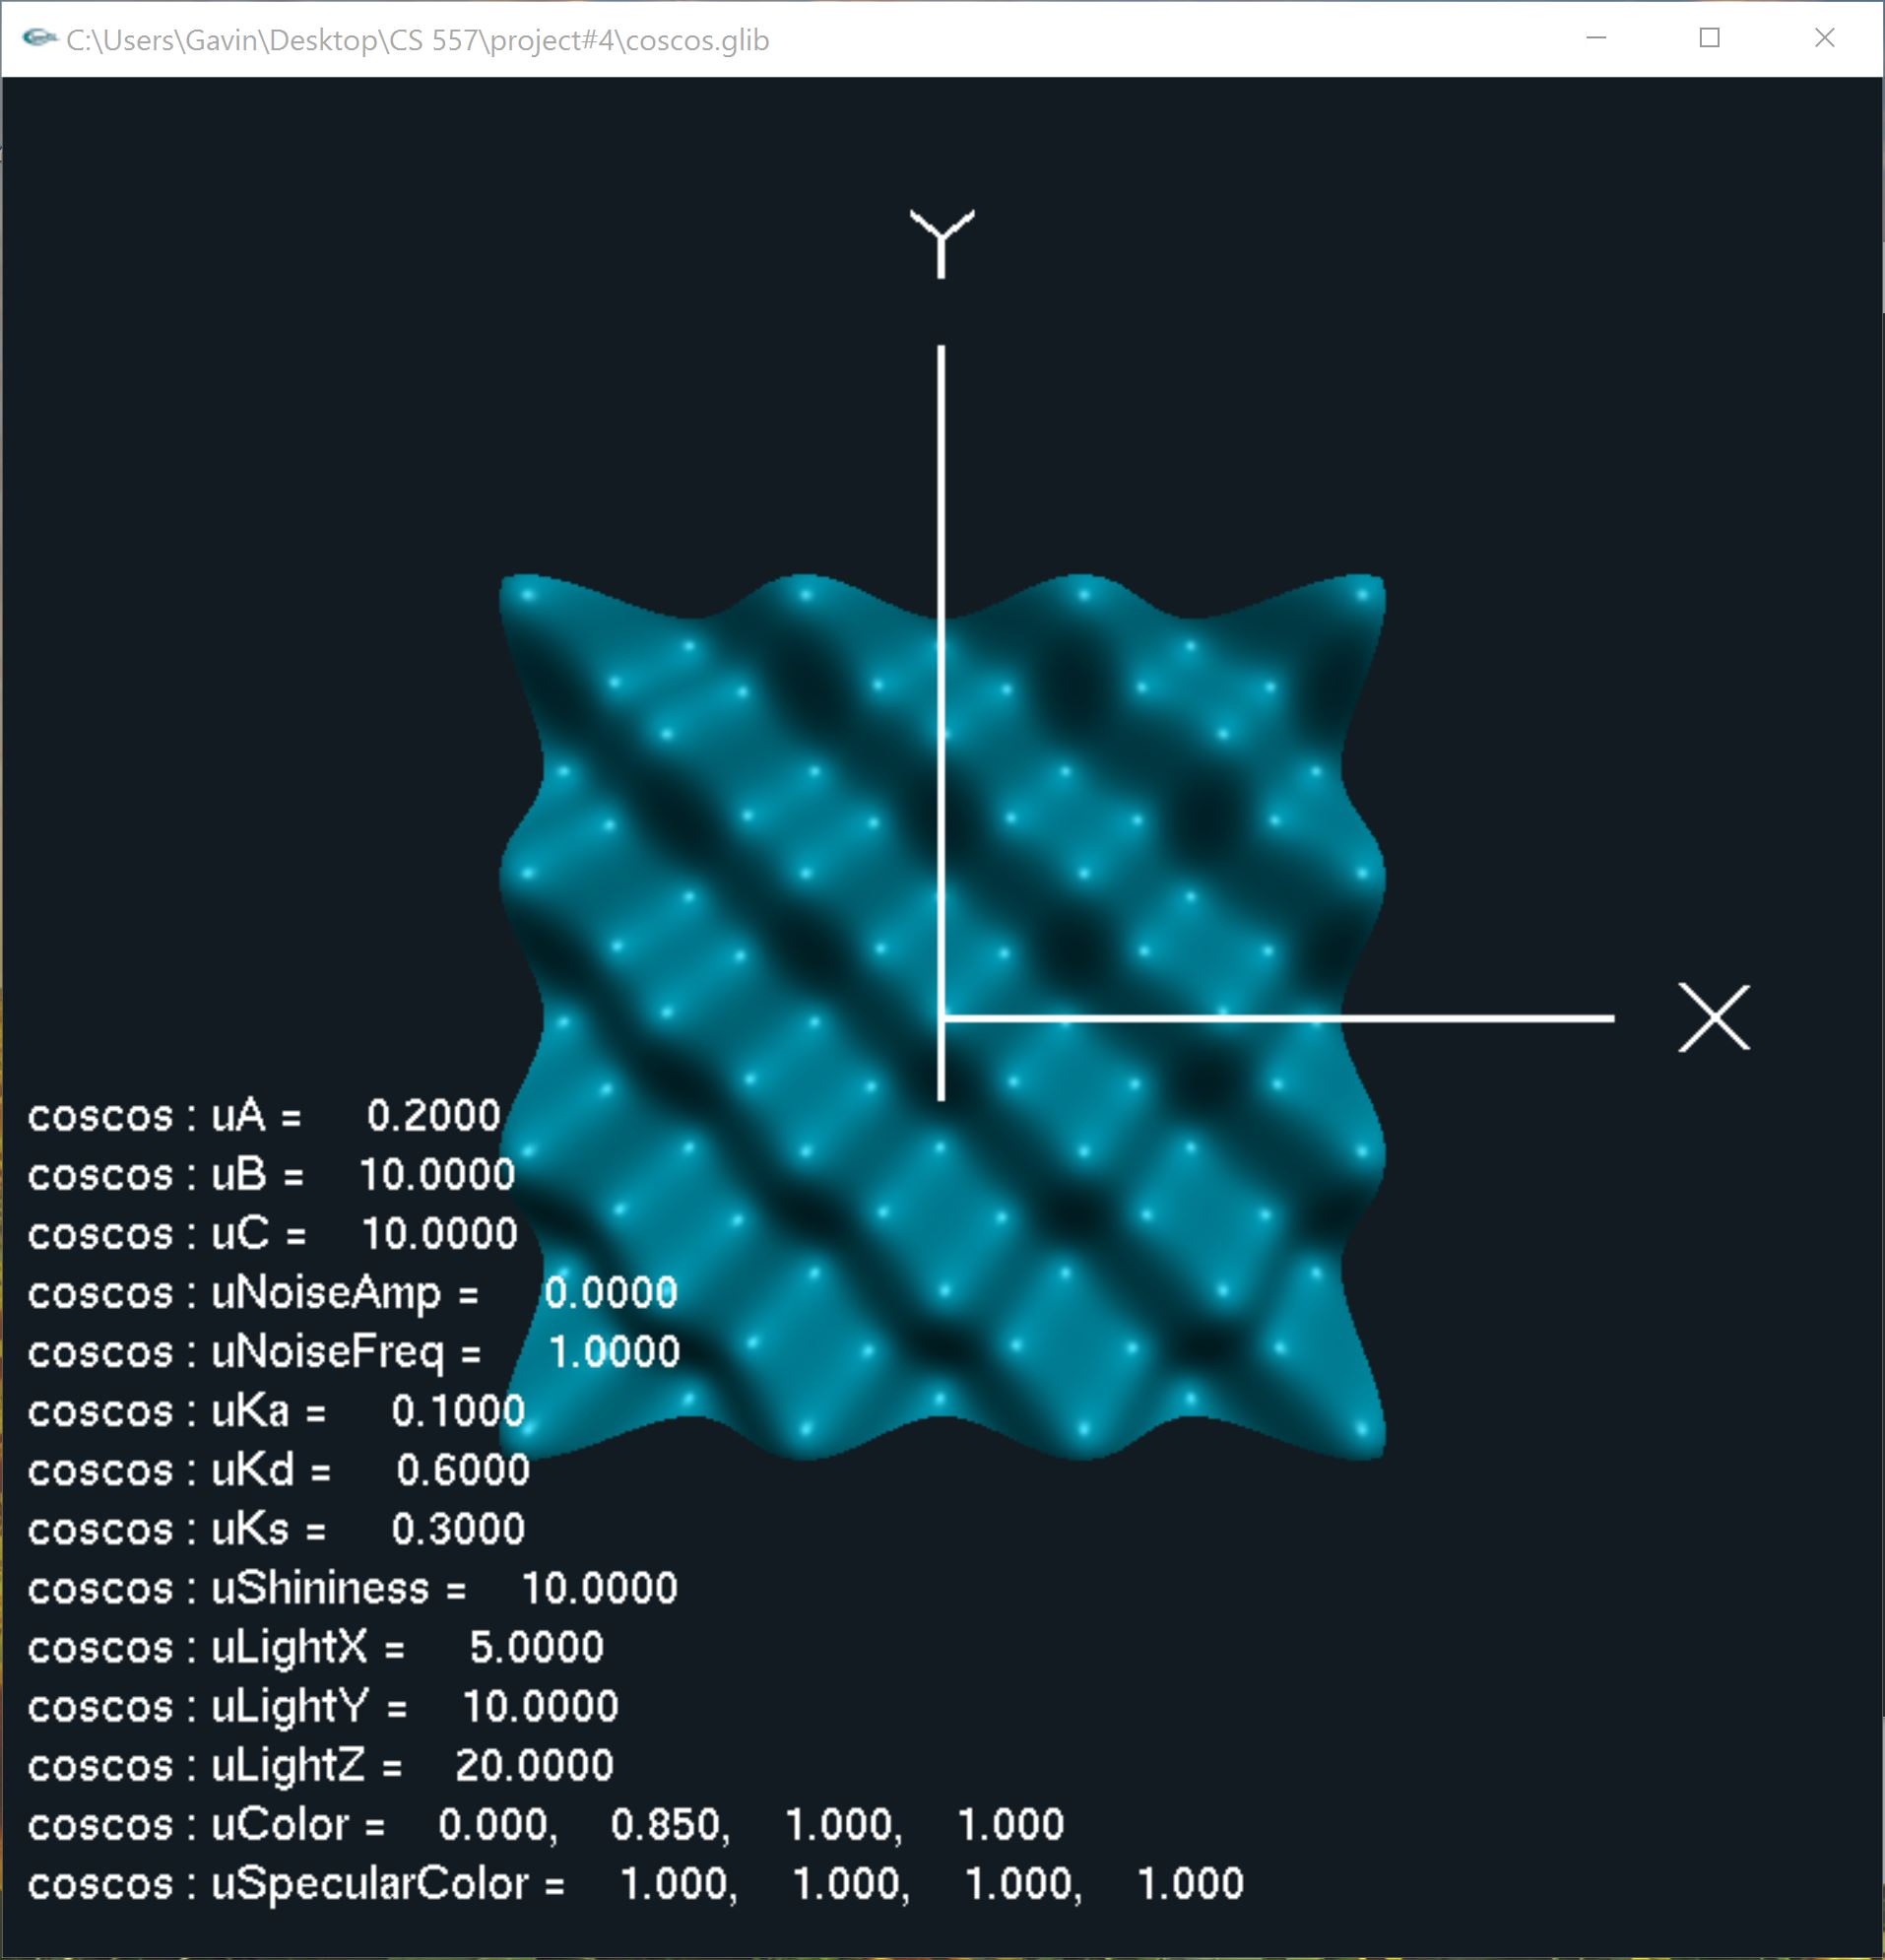
\includegraphics[width=5.5in]{origin.jpg}
\end{center}
The \textit{uAd} and \textit{uBd} sliders control the two diameters of the ellipse dots. In the RenderMan, we have to change these two values manually in the files, but thanks to the GLSL, we can control them by using two sliders. The first two sliders control these two parameters. The following two images show the examples of what will happen when manipulating these two sliders.
\begin{center}
	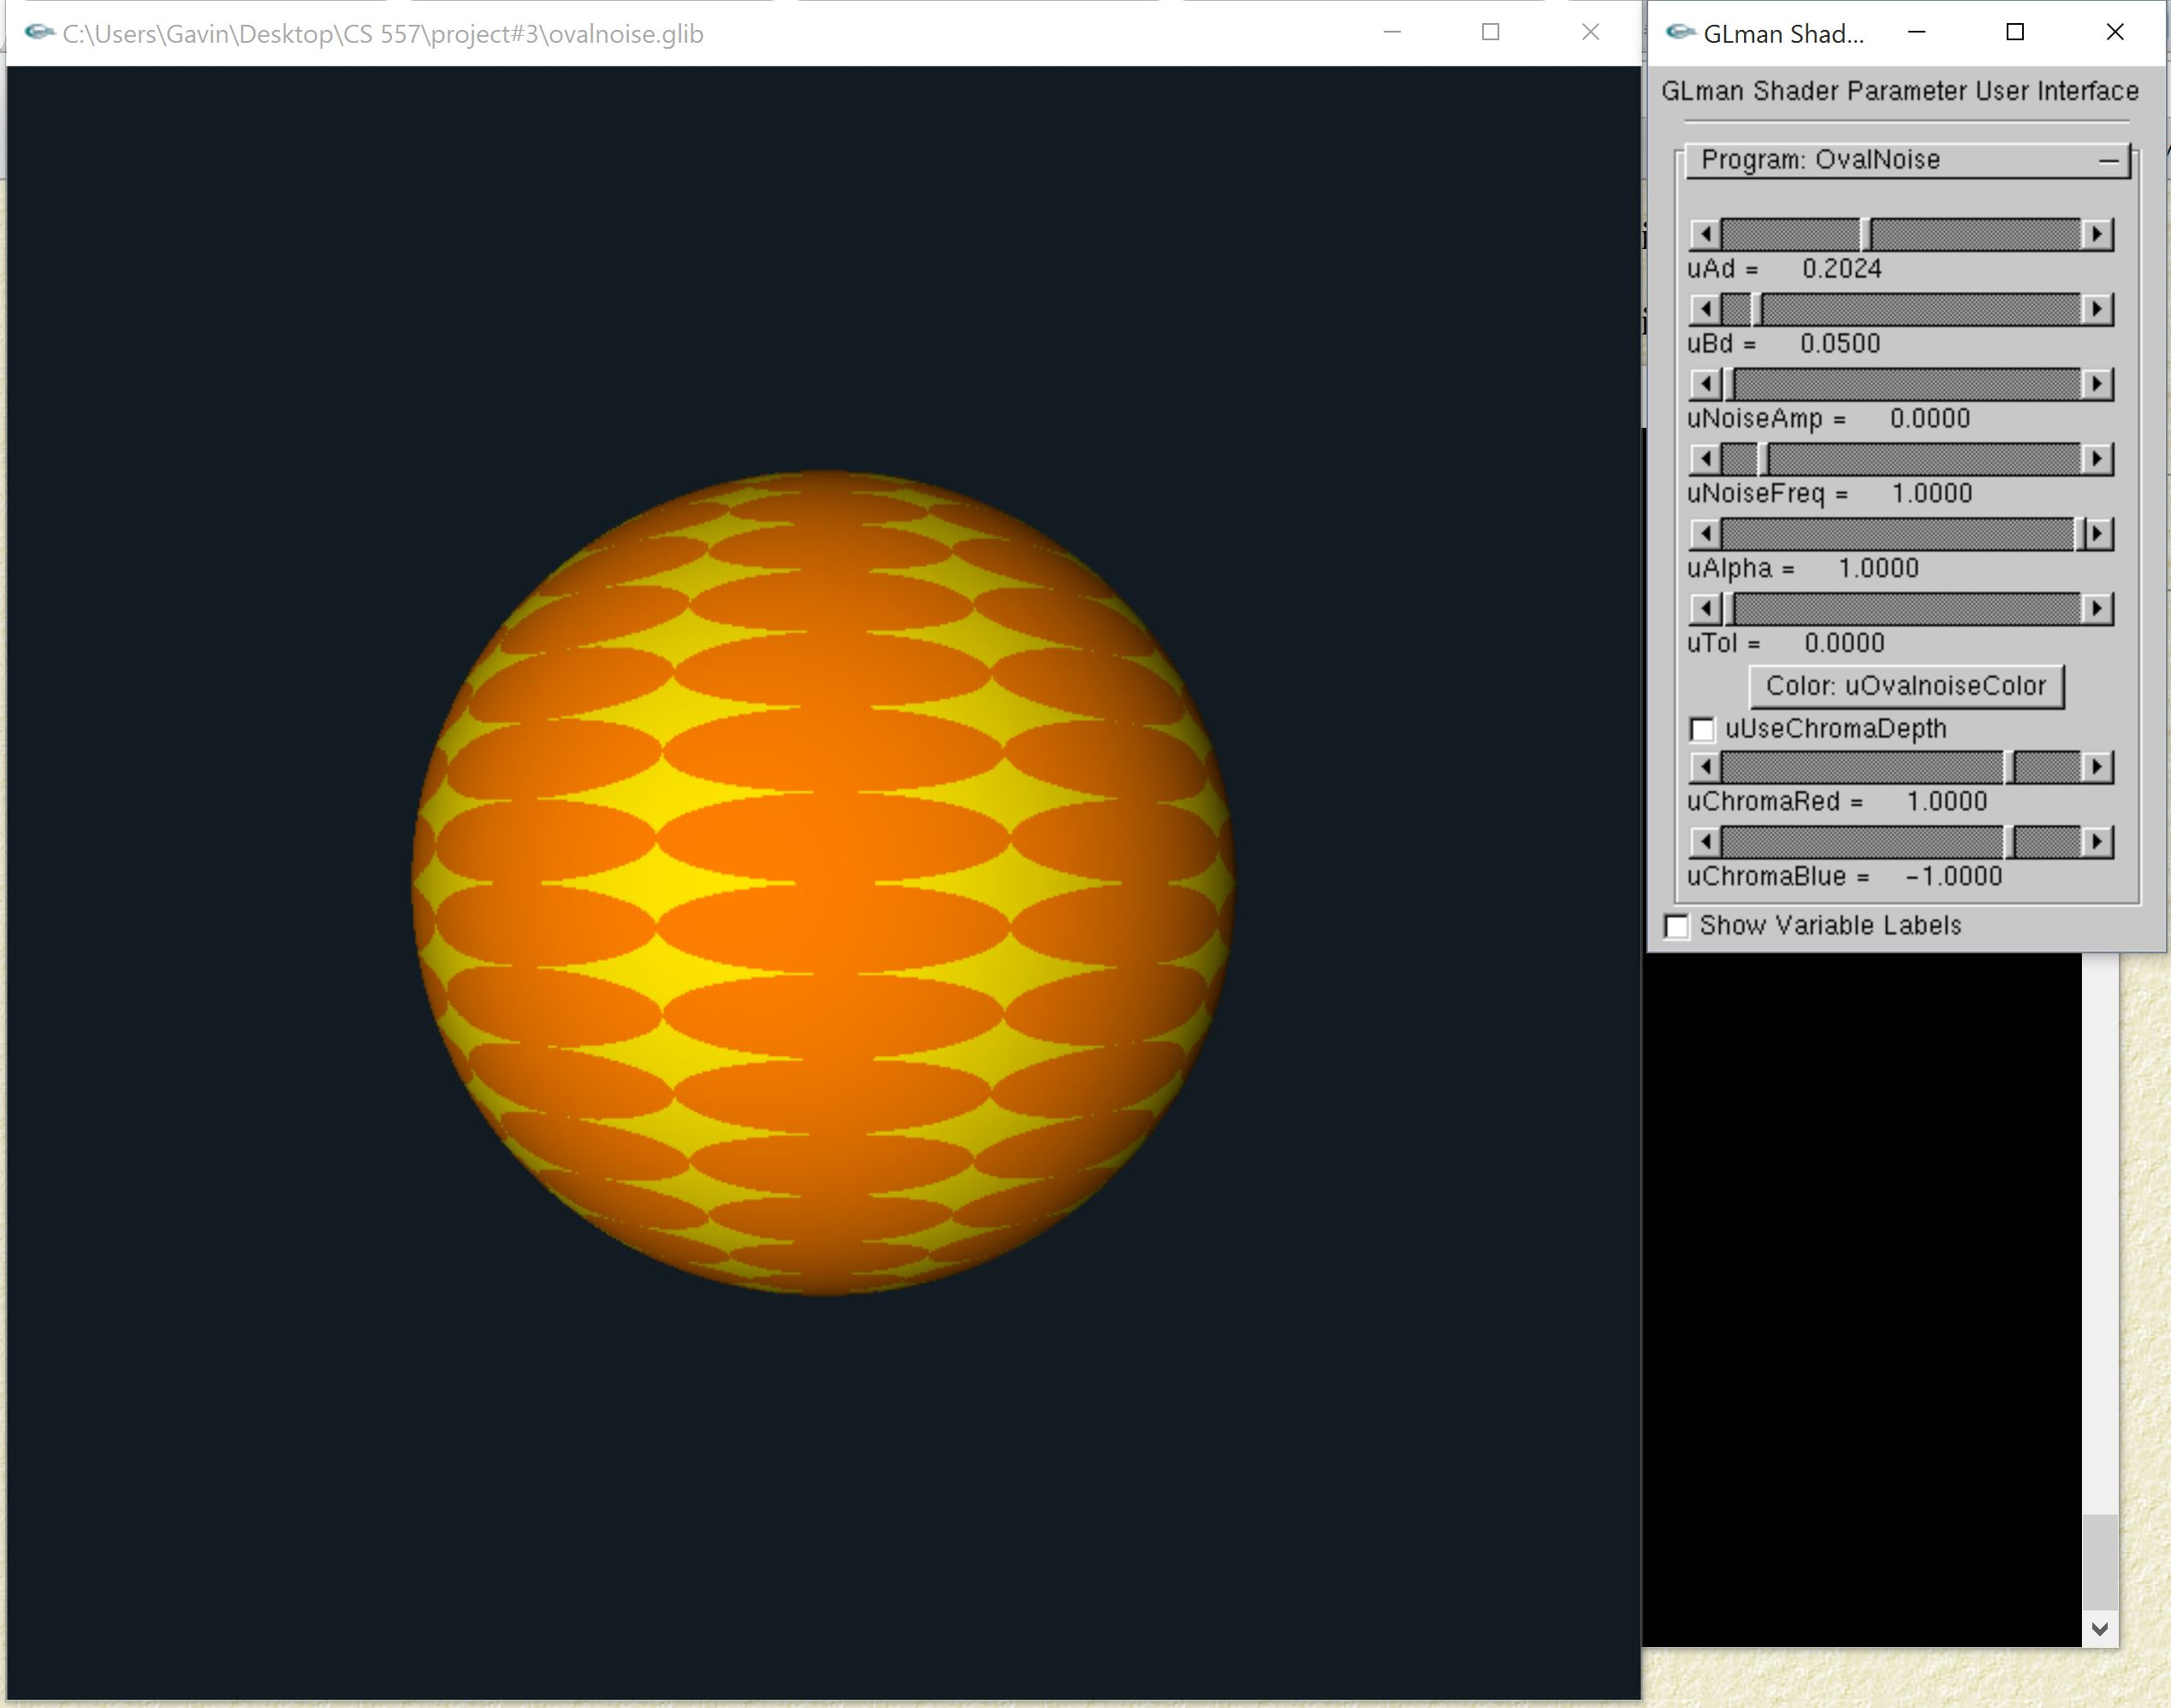
\includegraphics[width=3.2in]{AB1.jpg}
	\includegraphics*[width=3.2in]{AB2.jpg}
\end{center}
The noise is also applied to this project. The way to implement the noise using GLSL, is also pretty similar to the RenderMan noise. By following the equation $N = NoiseMag * noise( NoiseFreq * PP )$, the noise can be implemented easily. The two coefficients in this equation is controlled by two sliders. The $NoiseMag$ is replaces by $uNoiseAmp$, which is the third slider on the window. The $NoiseFreq$ is controlled by $uNoiseFrep$ which is the forth slider. The $uNoiseAmp$ controls the noise amplitude and the result is shown in the below left image. The $NoiseFreq$ controls the noise frequency and the result is shown in the below right image.
\begin{center}
	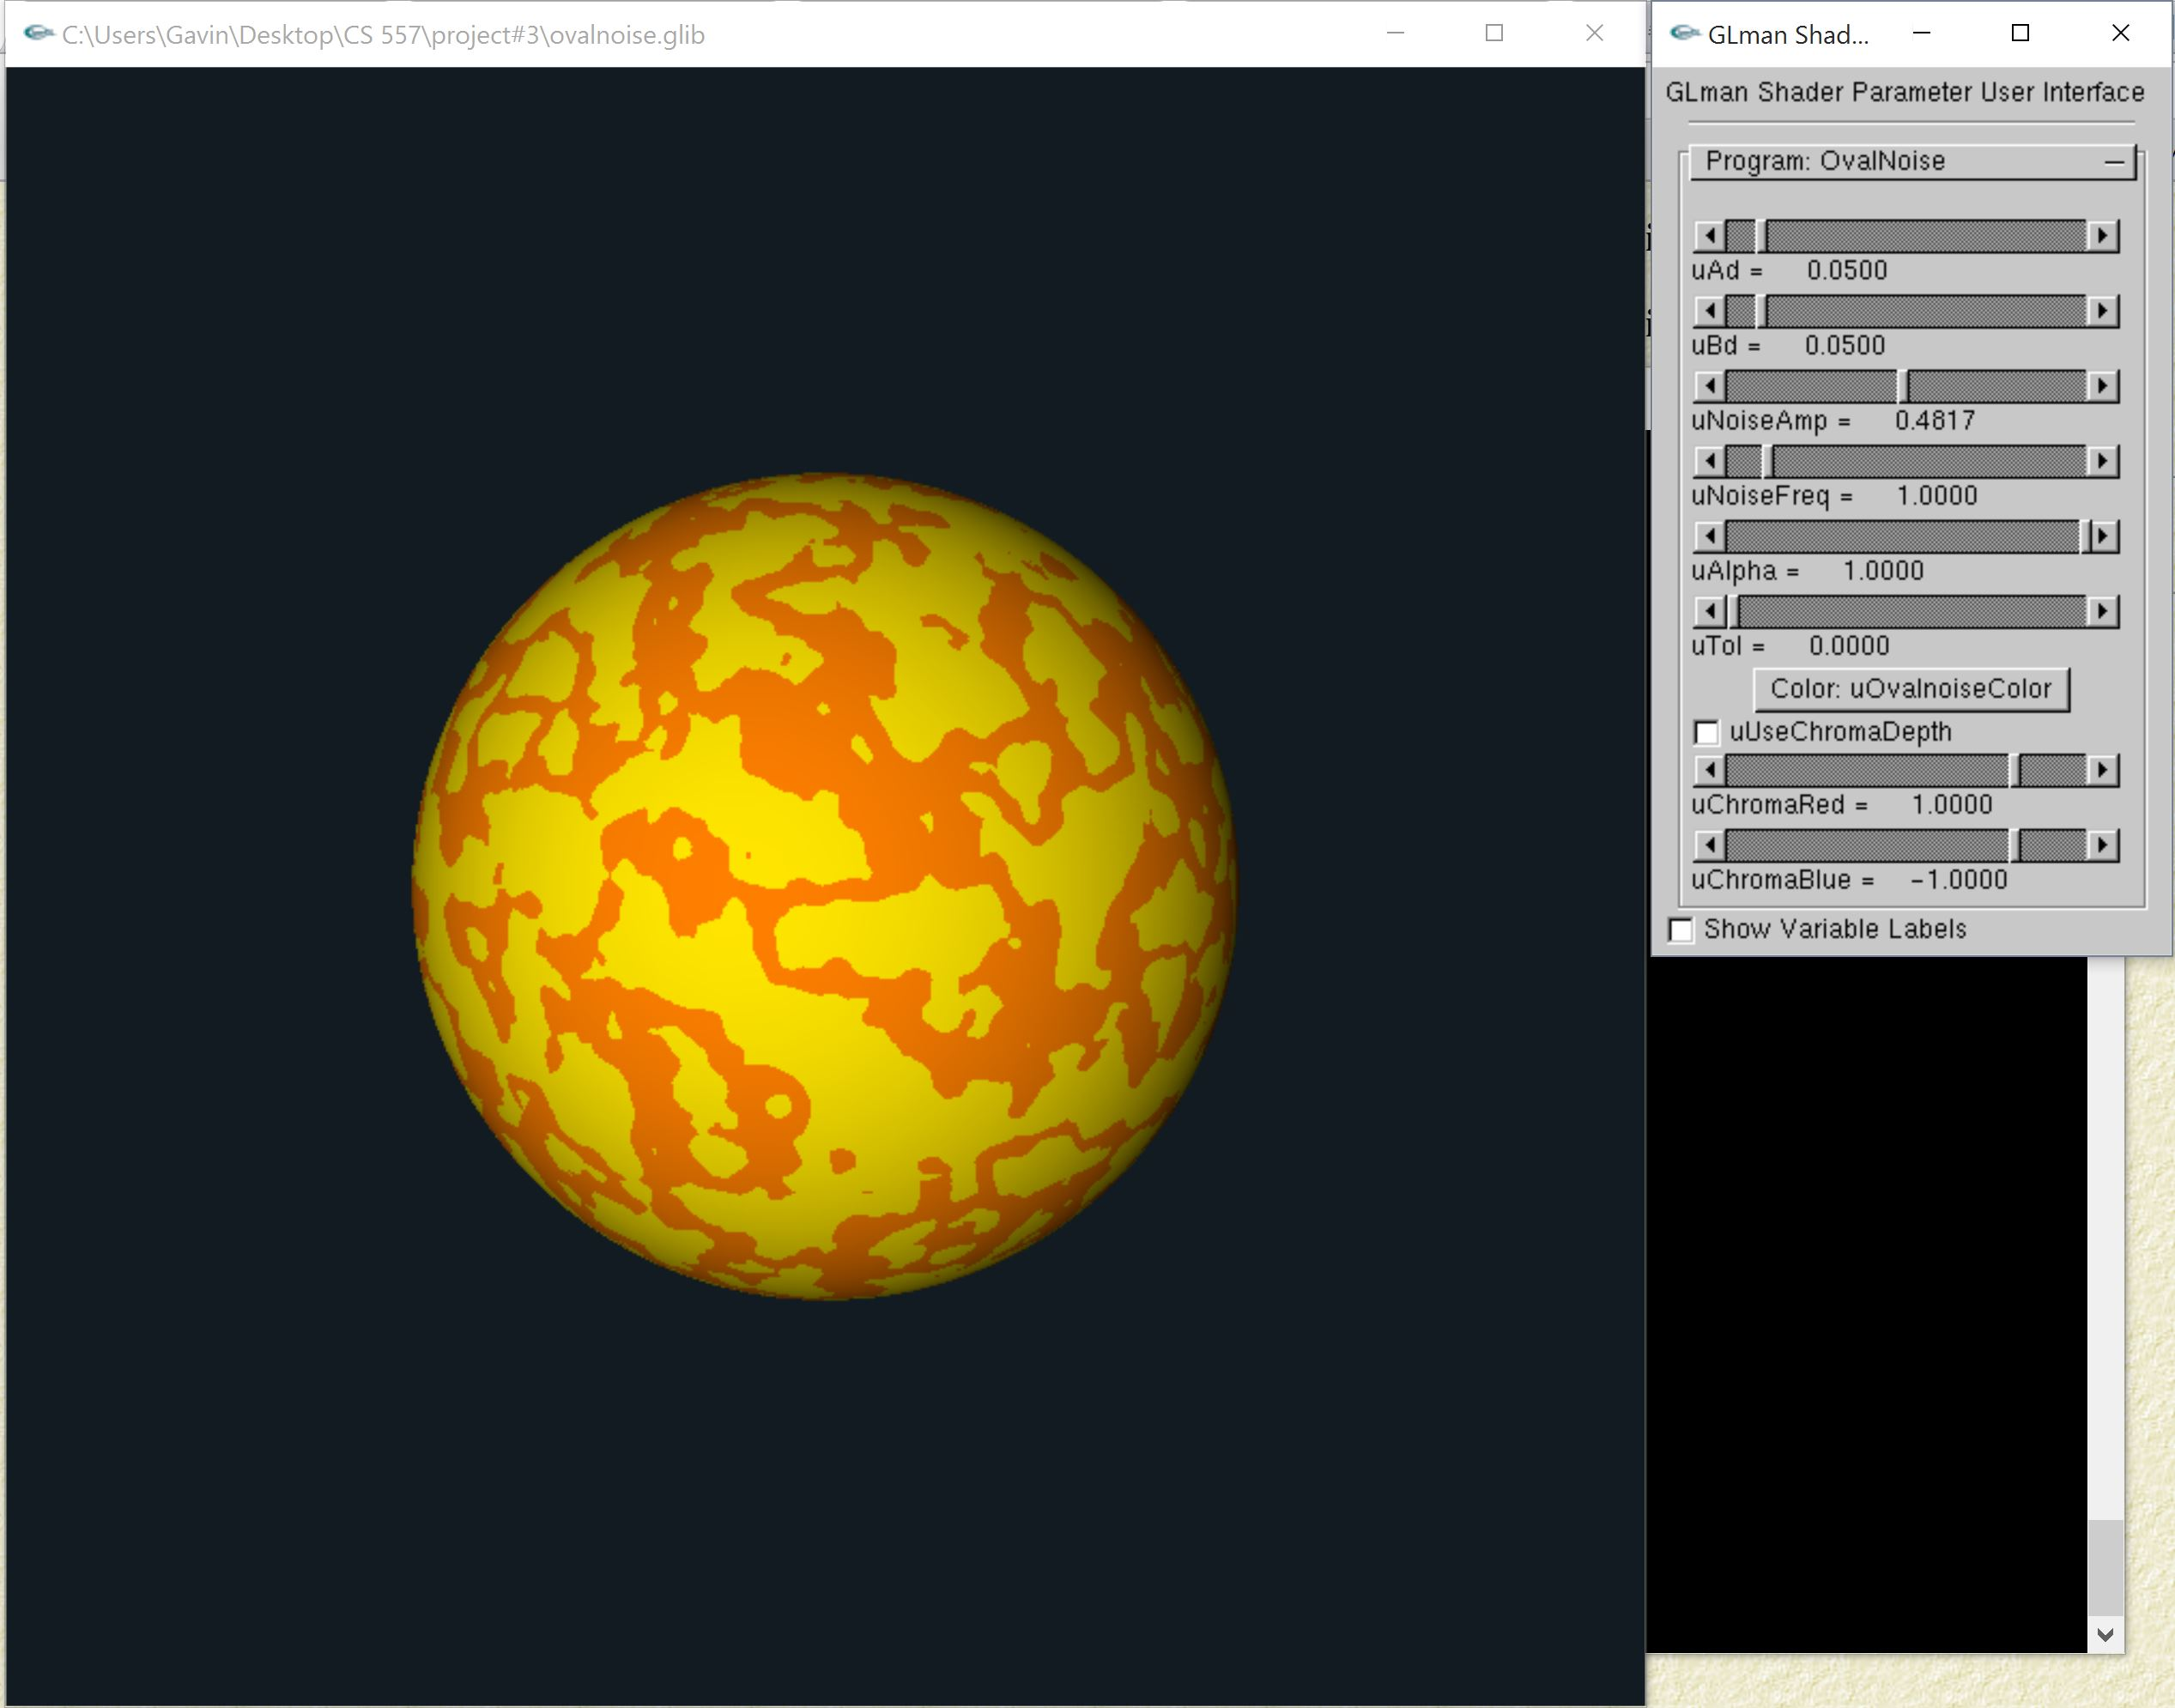
\includegraphics[width=3.2in]{NA.jpg}
	\includegraphics*[width=3.2in]{NF.jpg}
\end{center}
One new feature that has been added into this project is the tolerance. The tolerance has been implemented for both situations that with or without noise. The parameter that controls the tolerance is changed by a slider named ``uTol''. To implement tolerance, as for this project, I just added and subtracted tolerance value to the boundary value $1$, and put these two values into a \textit{smoothstep} function in order to set the range for the colors to get mixed together. Then by putting the range and the two colors together into the \textit{mix} function, the smooth change in between two colors around the edge will be created. The following two images show the results for adding the tolerance to the pattern on the sphere with and without noise.
\begin{center}
	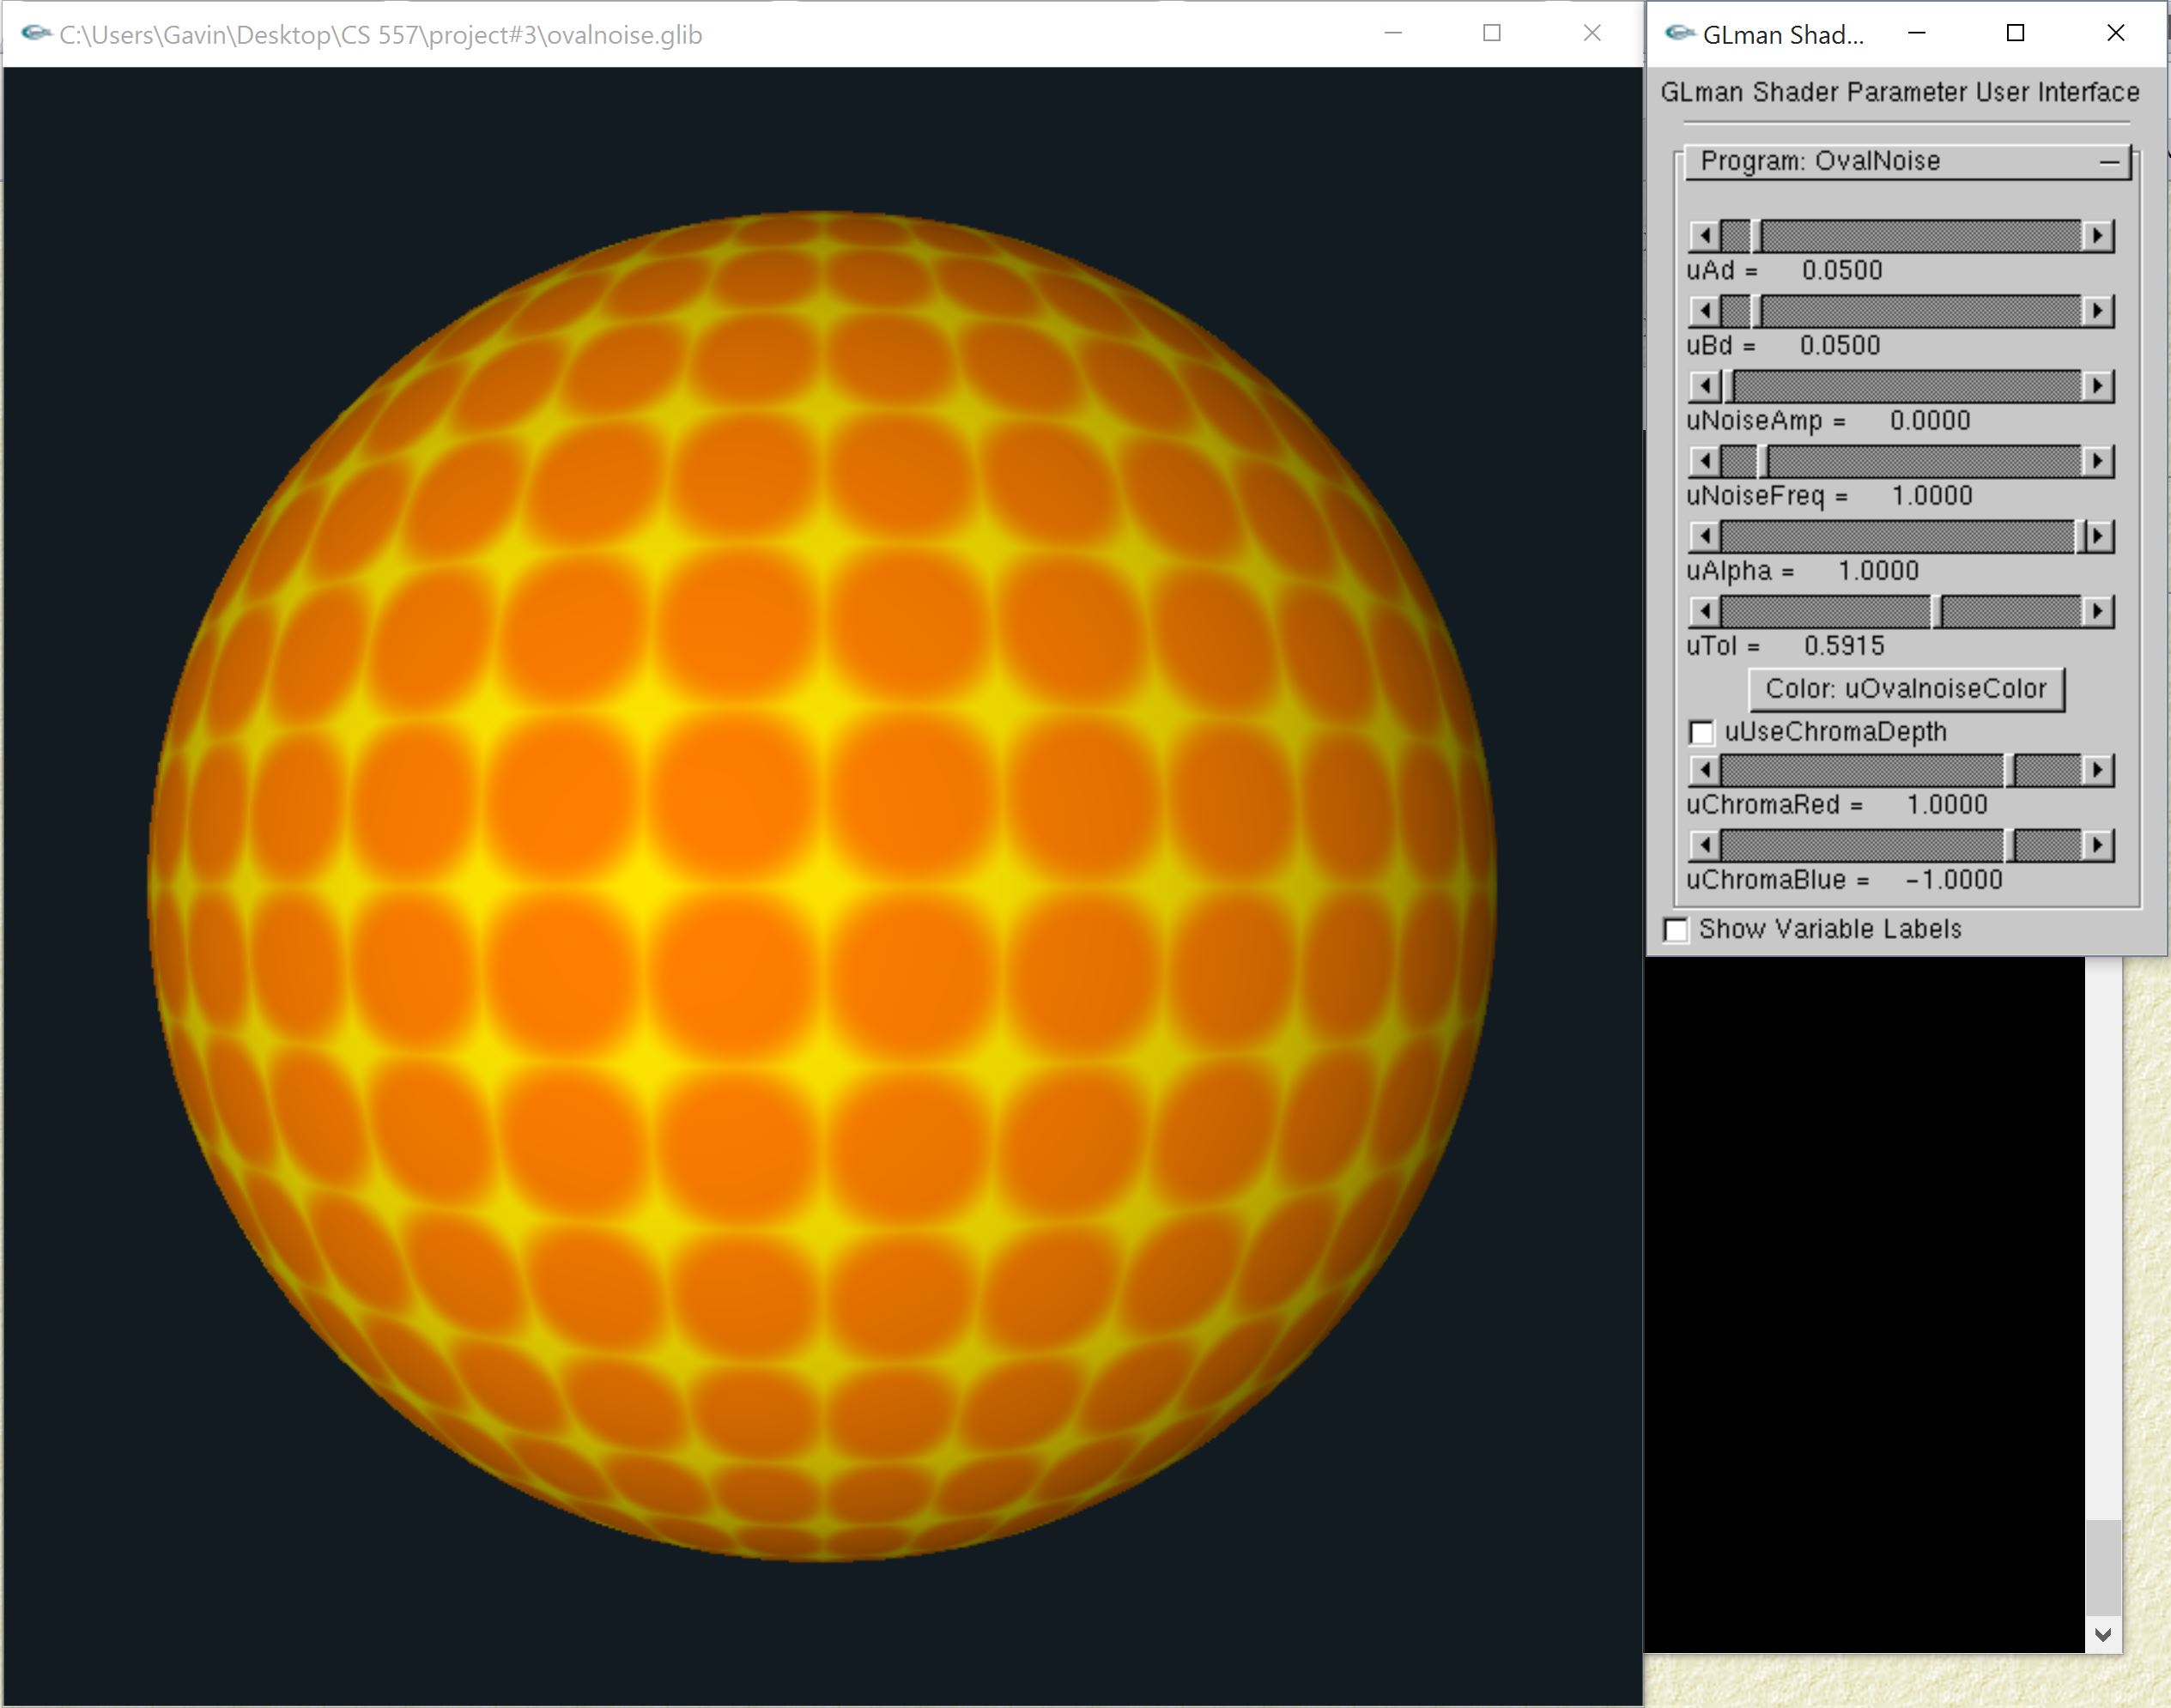
\includegraphics[width=3.2in]{T1.jpg}
	\includegraphics*[width=3.2in]{T2.jpg}
\end{center}
At this point, all of the requirements of the project have been accomplished and explained. The following part of the report will talk about two extra credits of the project.

The first extra credit is implementing the transparency on the sphere surface along with the noise. In the requirement of this exta credit, when the alpha value is between 0 and 1, we can simply add the alpha into account with the RGB, this will result in some part of the sphere cannot be shown properly. When the opacity is set to 0, then we should simply do the ``discard'' instead of setting the alpha to 0, and this will give us a good looking sphere without any problem. The images below show the result of that. The one on the left is doing with alpha value, and the back upper part of the sphere is black. The one on the right is using discard, and the back upper part turns out to be correct. The opacity is controlled by a slider named \textit{uAlpha} in the interface.
\begin{center}
	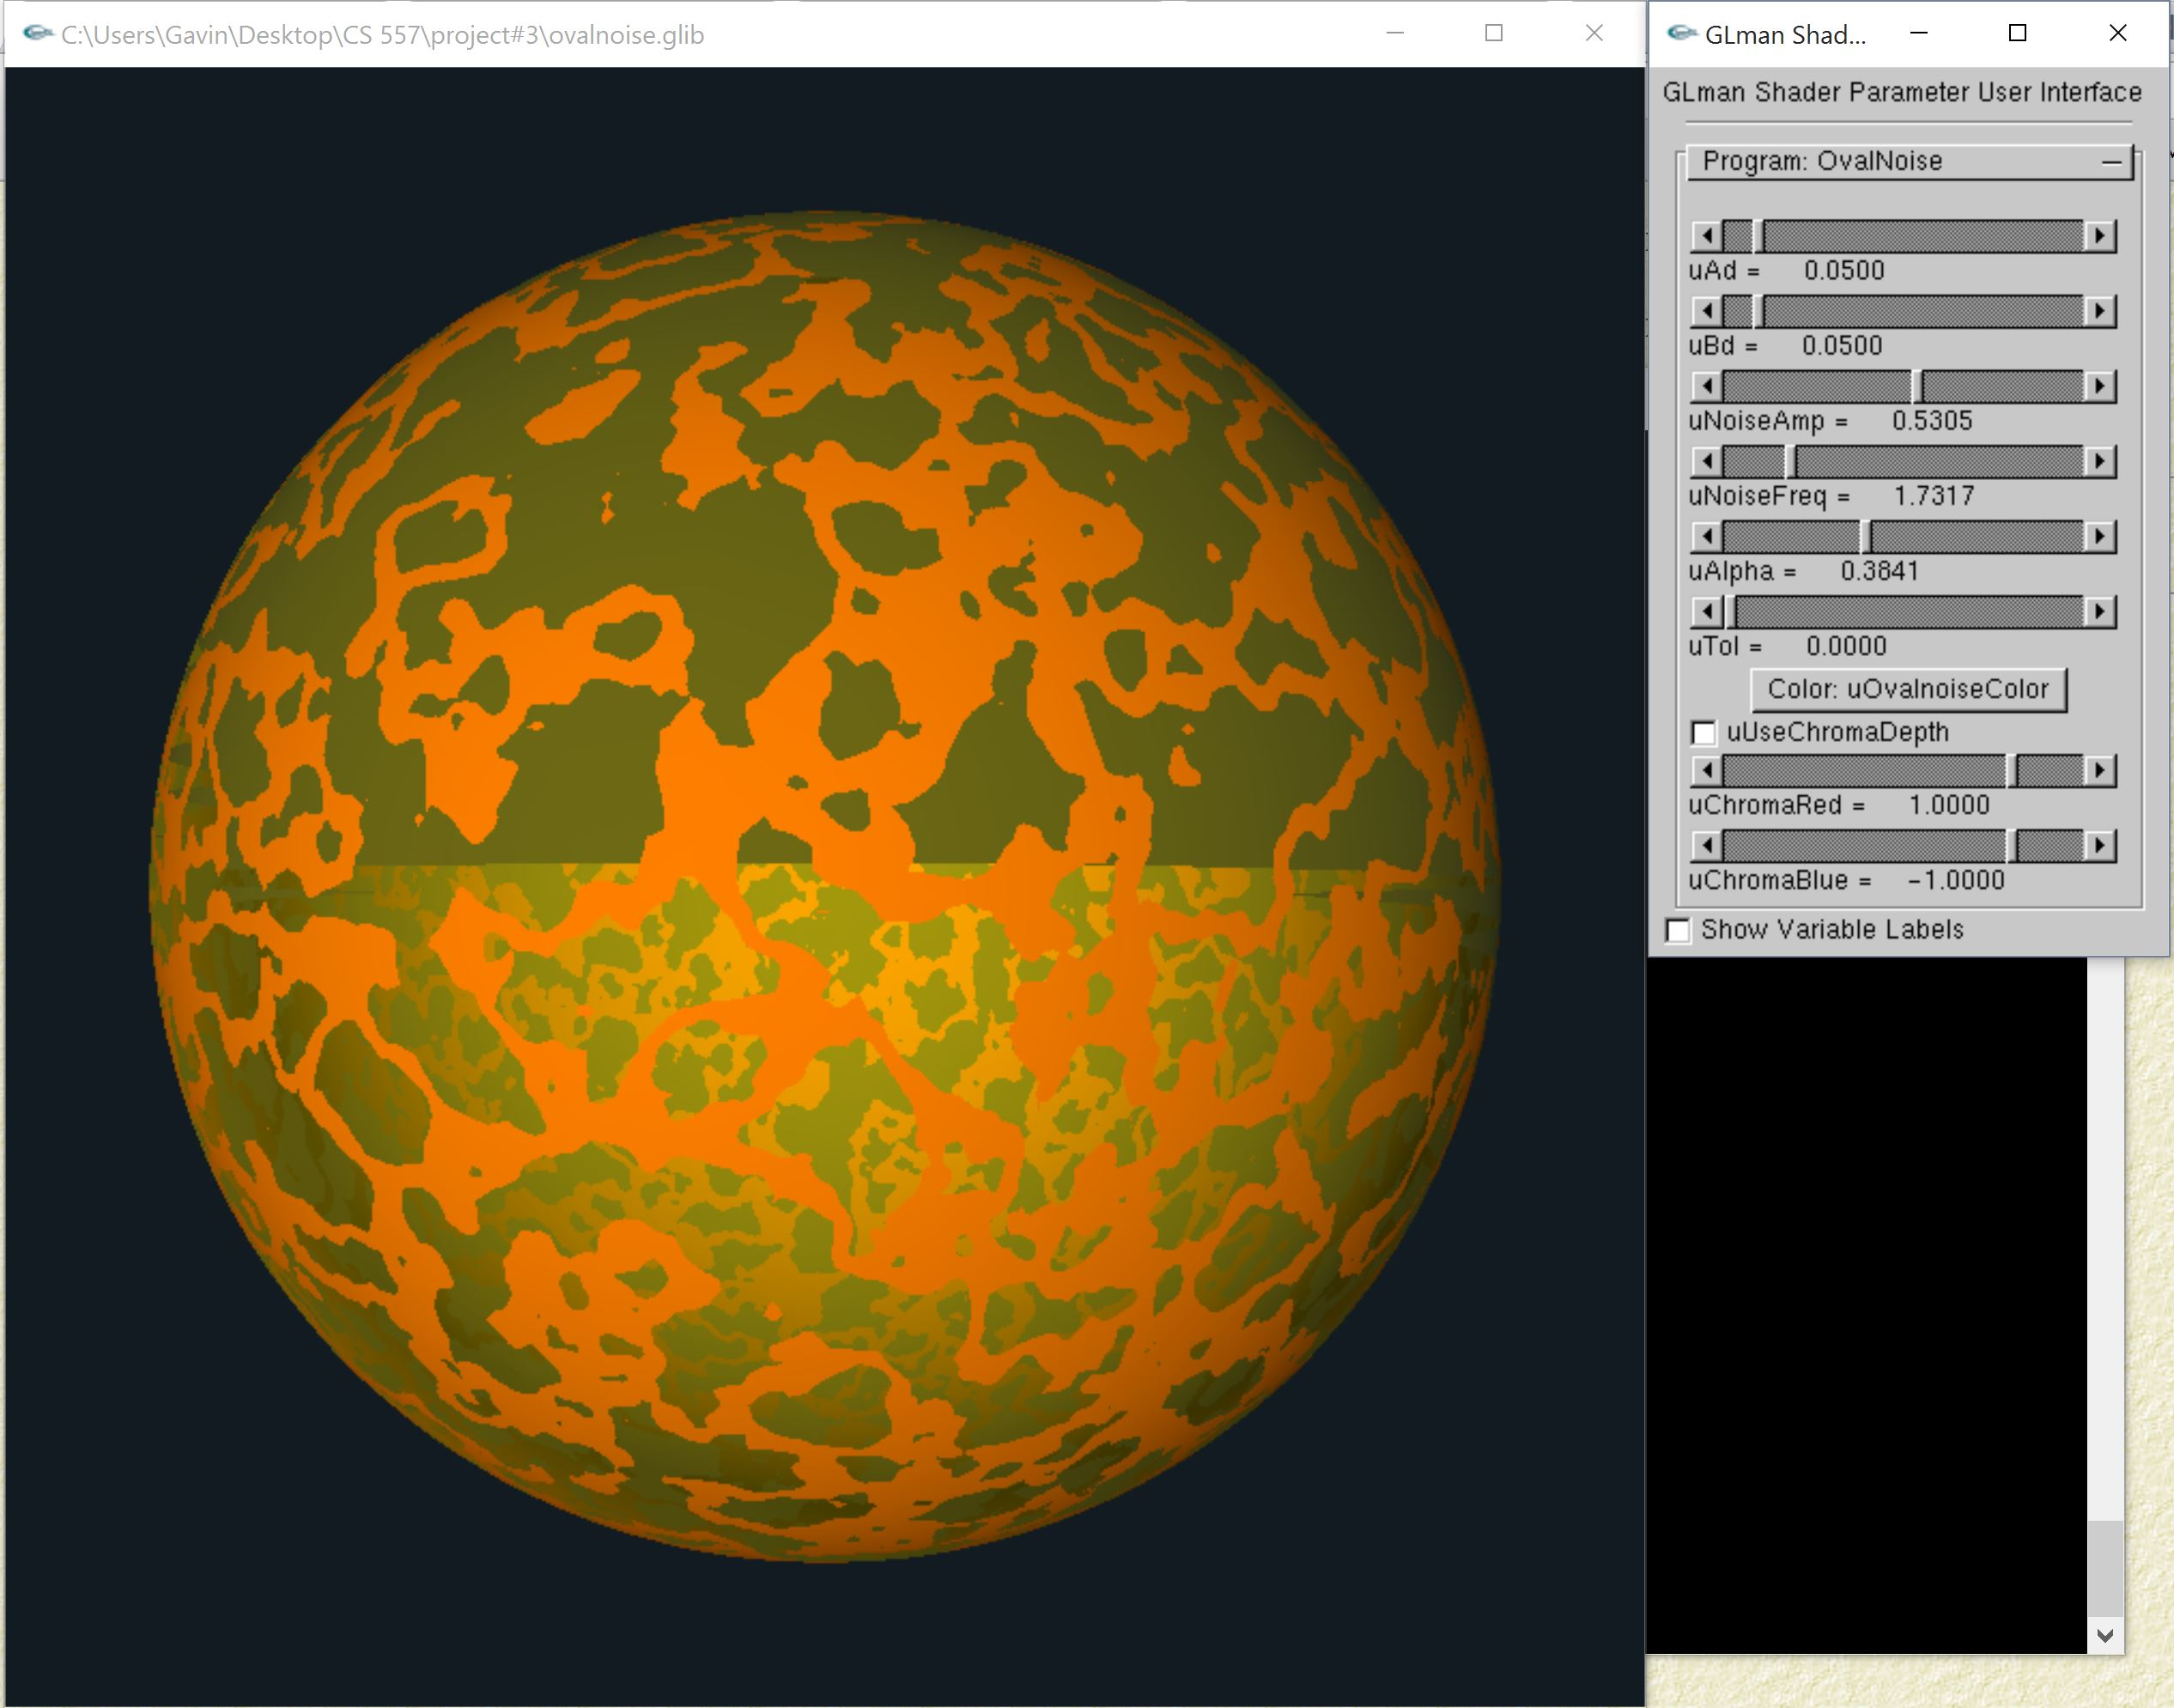
\includegraphics[width=3.2in]{E11.jpg}
	\includegraphics*[width=3.2in]{E12.jpg}
\end{center}
The second extra credit is implementing the ``ChromaDepth'' feather into the project. The ChromaDepth does the job that rendering the closer part of the object to red and the further part of the object to blue. So that we need to keep the closer part always be rendered as red no matter how the object id rotated of transformed. In order to implement this, we need to change the model coordinate into world coordinate. This is easy to do, just multiply the ``gl\_ModelViewMatrix'' with the model coordinate in the vertex shader will do the trick. The red range and the blue range in the image are controlled by two sliders named \textit{uChromaRed} and \textit{uChromaBlue}. In the following images, the axes is turned on in order to deliver the idea that the sphere has been rotated but the rad-blue range stays the same.
\begin{center}
	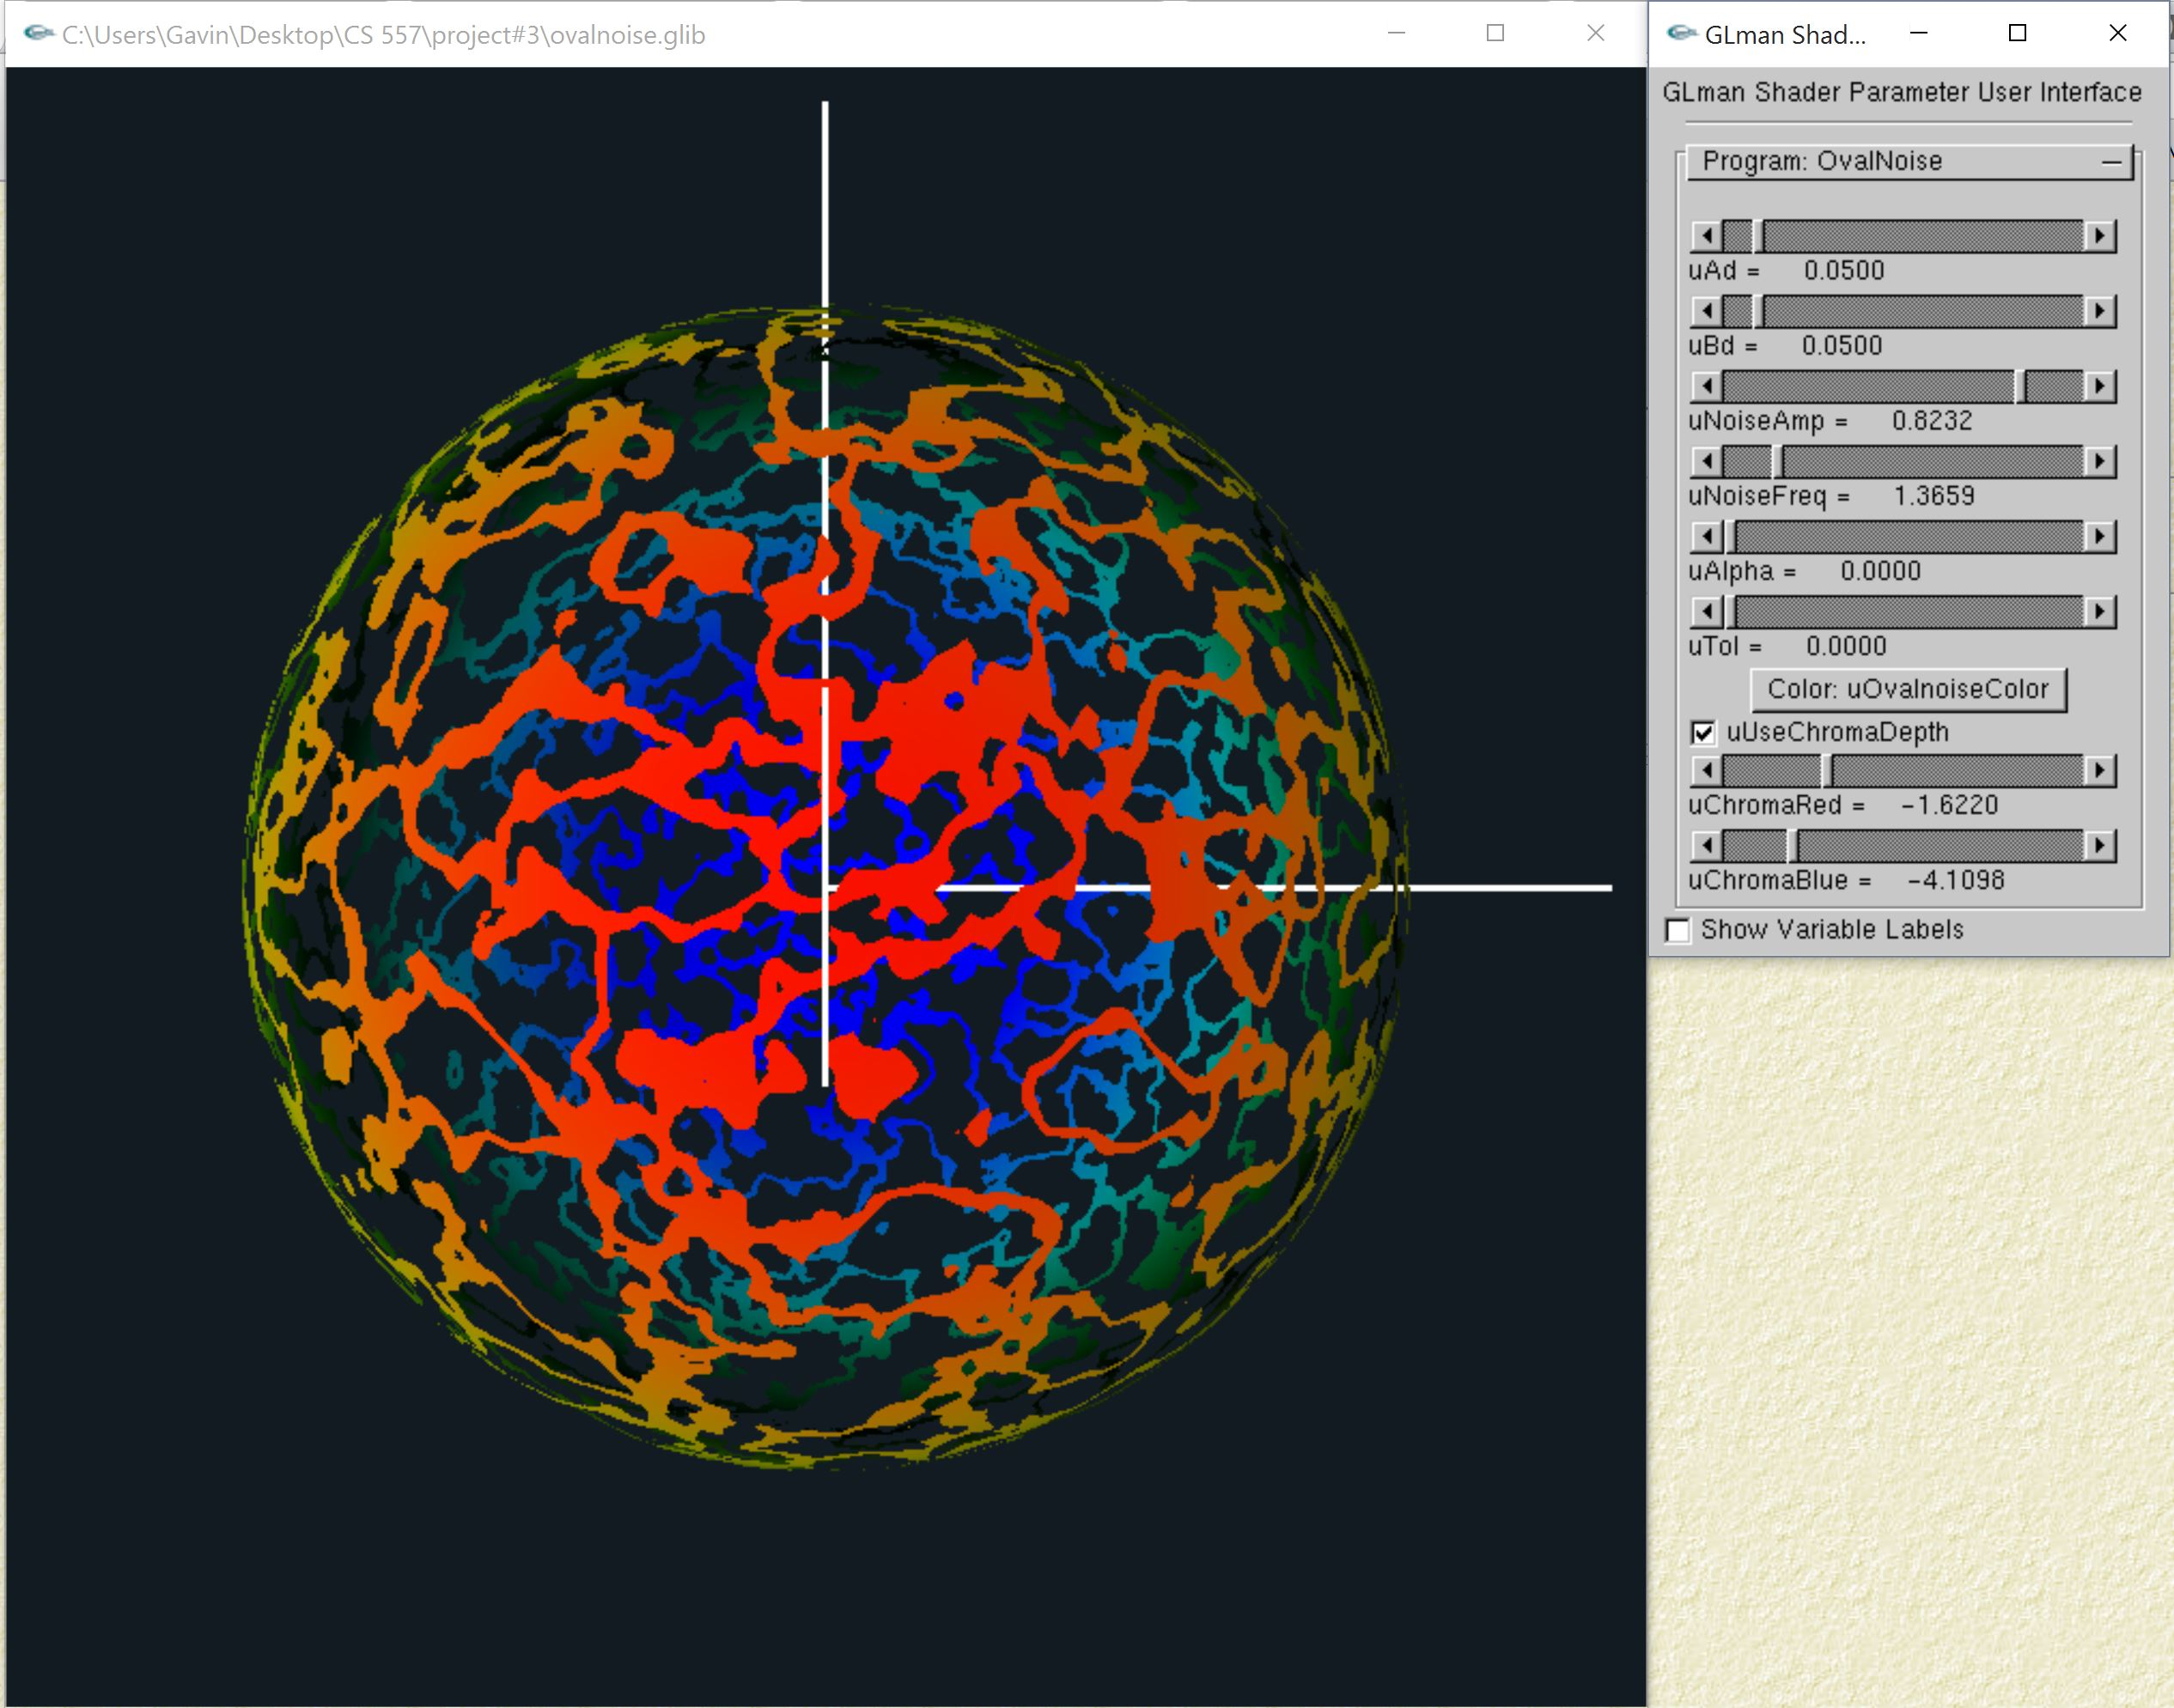
\includegraphics[width=3.2in]{E21.jpg}
	\includegraphics*[width=3.2in]{E22.jpg}
\end{center}
The ChromaDepth could work with a pair of special-made glasses to create a 3D effect. With the glasses on. the red part of the object will become closer to the viewer and the blue part will become further. This effect relates to the face that the glasses refract different colors' wave with different degrees. So looking into the sphere listed below with glasses on will result in a 3D scene.
\begin{center}
	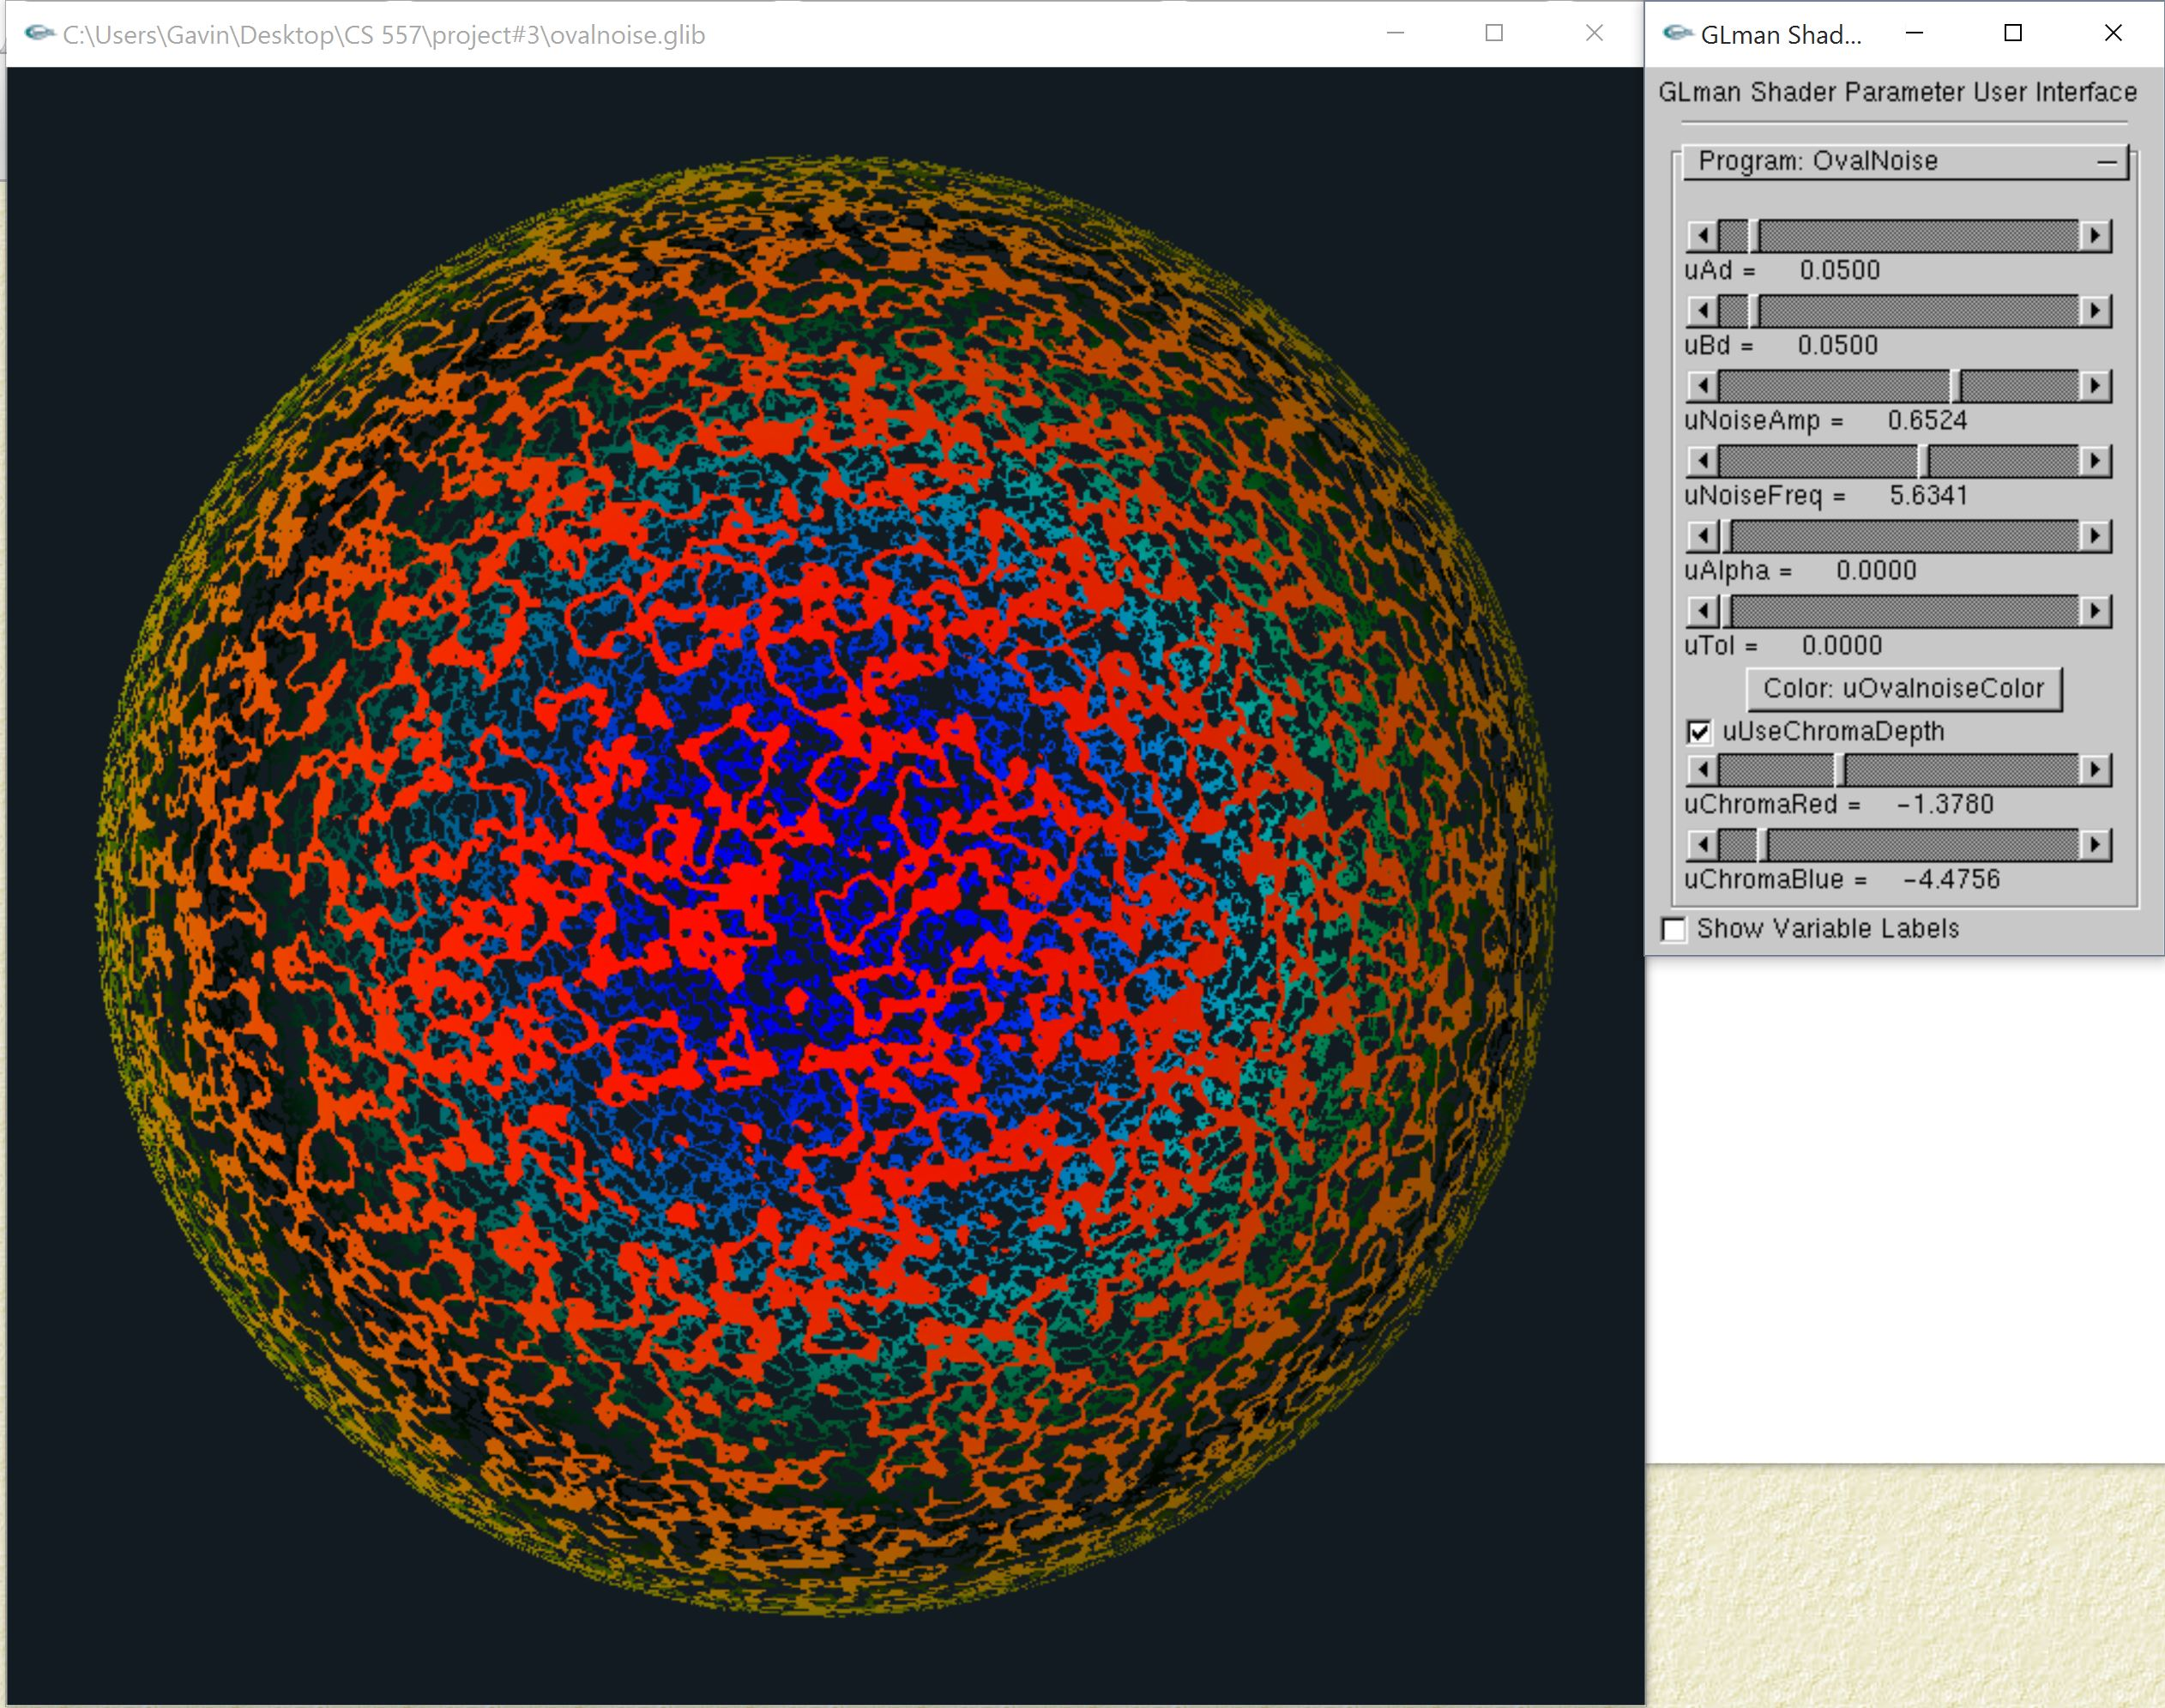
\includegraphics[width=5in]{E23.jpg}
\end{center}
Finally, by changing the object we put into the scene, we could have something really fun!
\begin{center}
	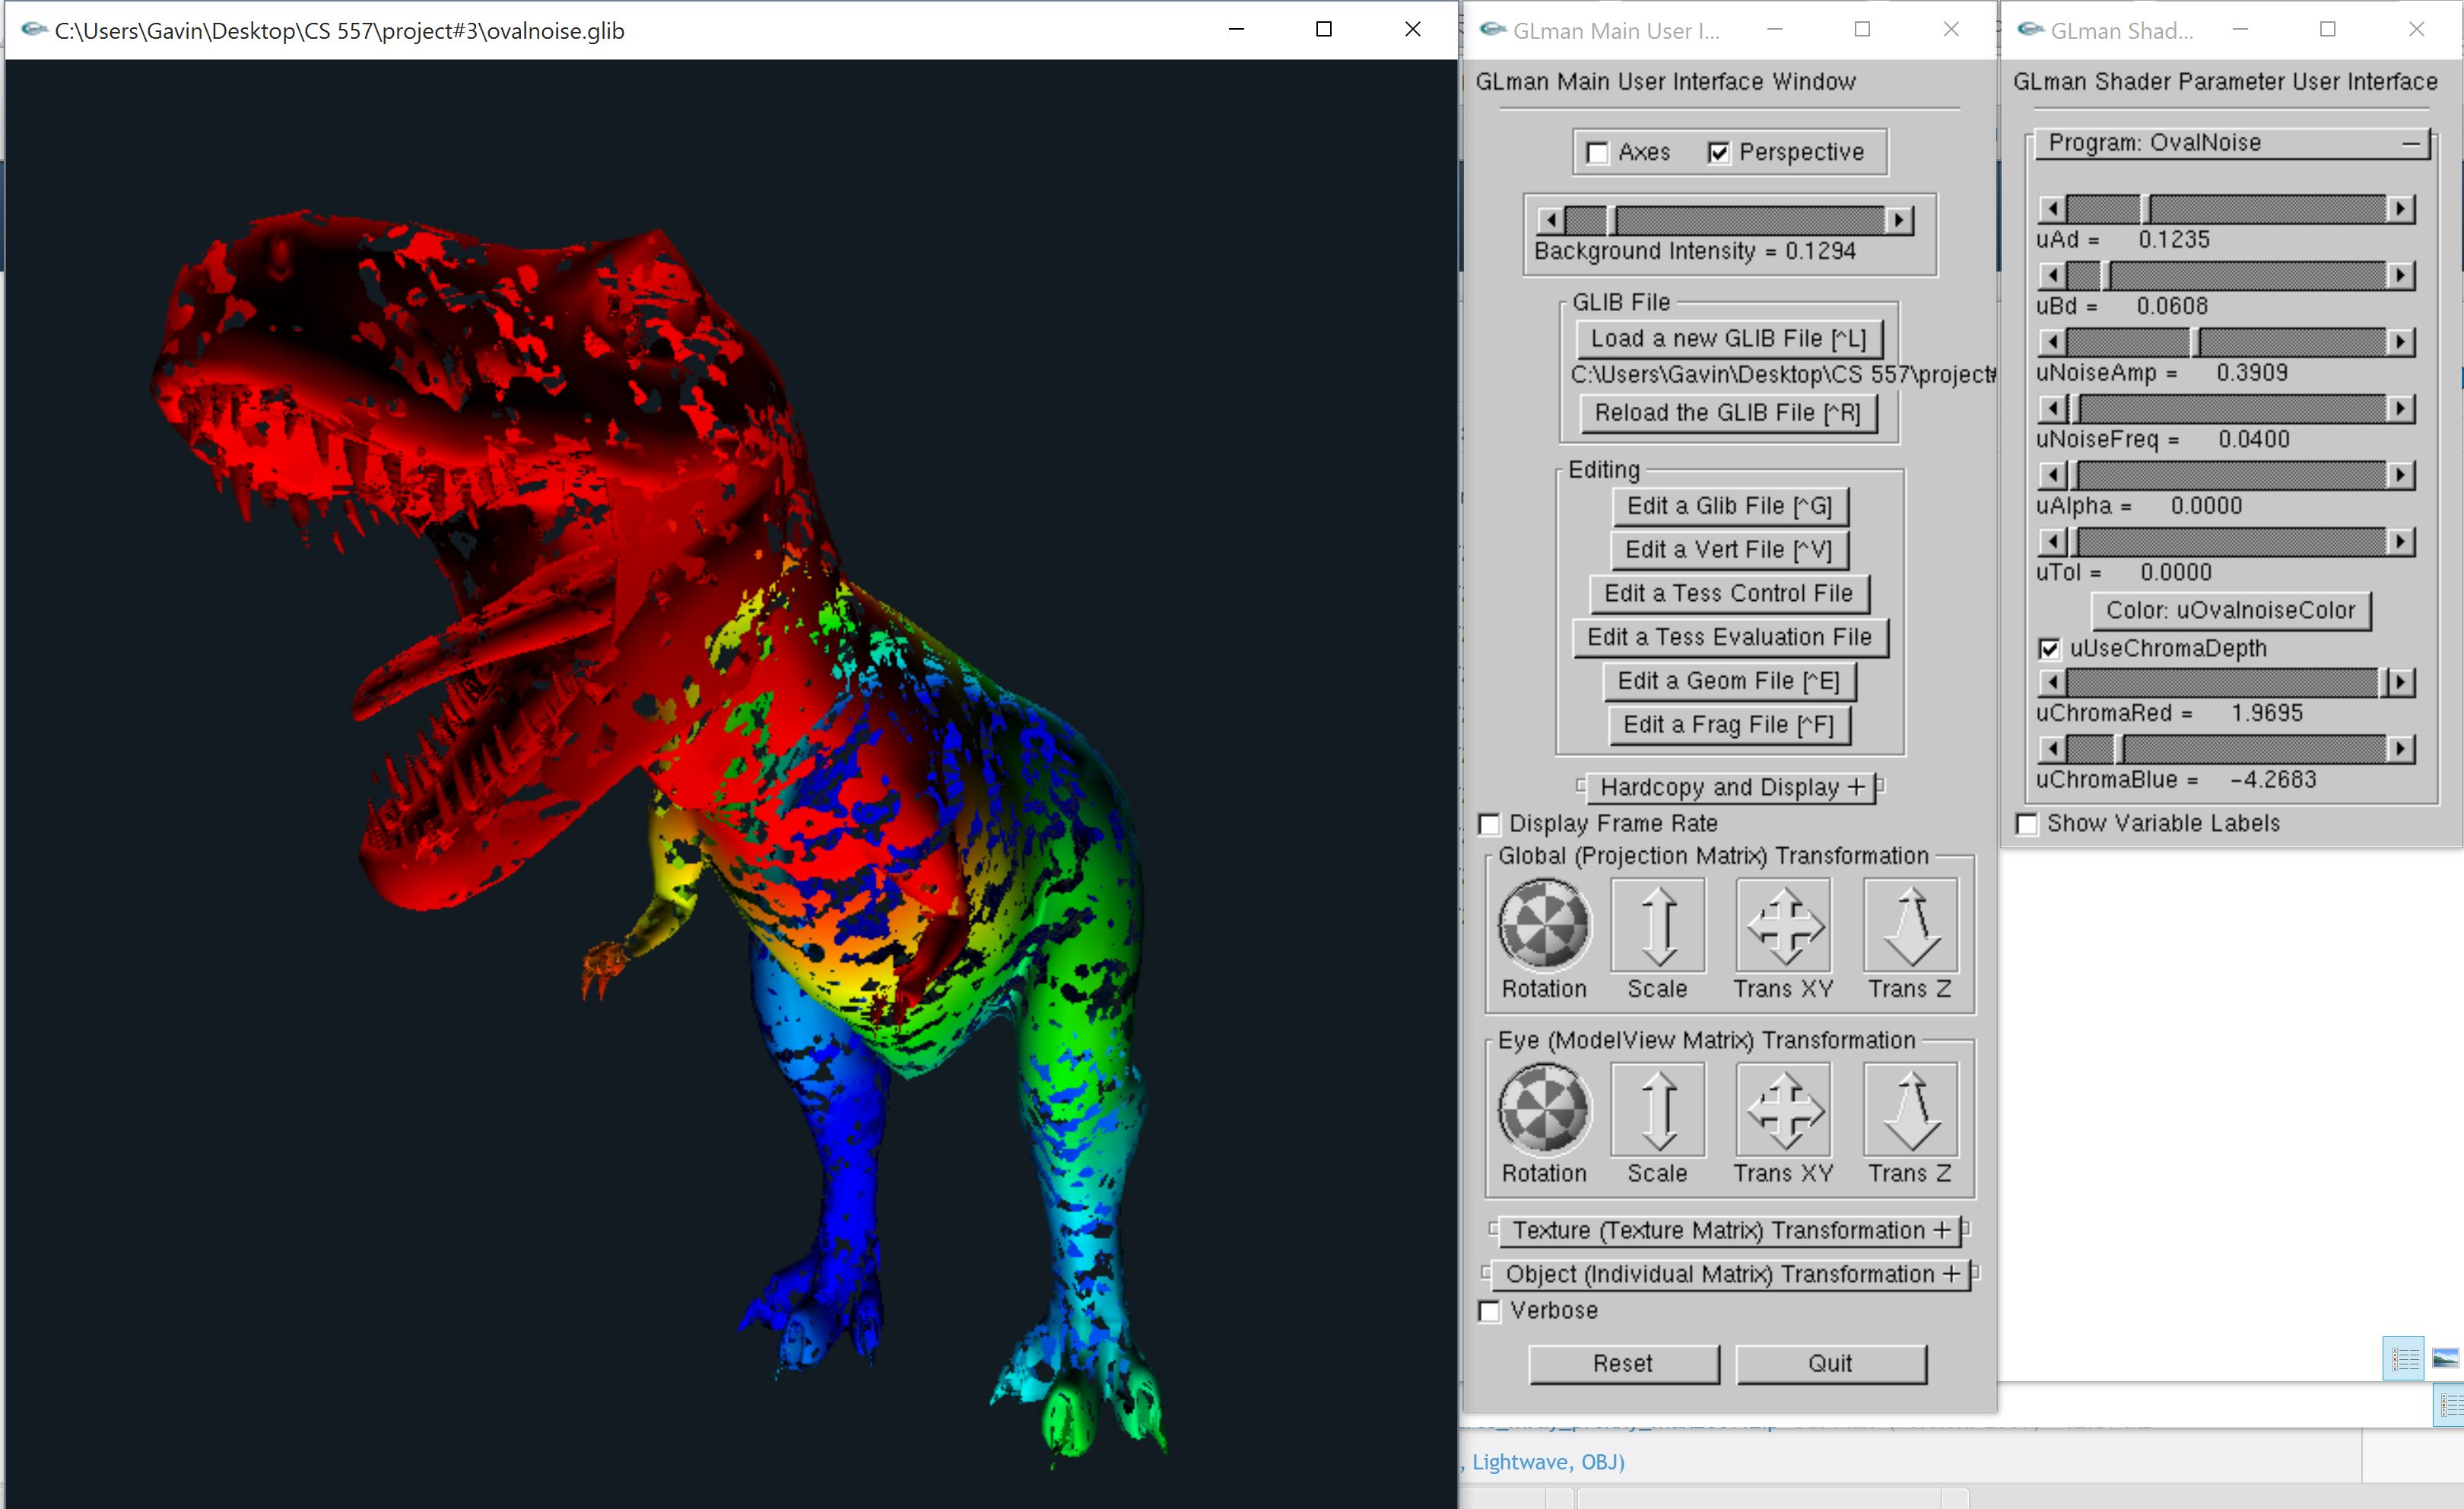
\includegraphics[width=5in]{FUN.jpg}
\end{center}
\section{Summary}
This project includes a lot of the knowledge that taught in the class and is really interesting. By doing this project, I got a pretty good review of the knowledge that need to be used in it and gained a better and deeper understanding on them. Playing with noise and some object files is also pretty fun and makes this project a lot more interesting. I'm looking forward to the following shader projects and willing to do a lot more on them.
\end{document}